\pagelayout{margin}
\setchapterstyle{kao}
\setchapterpreamble[u]{\margintoc}
\chapter{Research and implementation}
\label{ch:problem}

\begin{figure}[hb]
    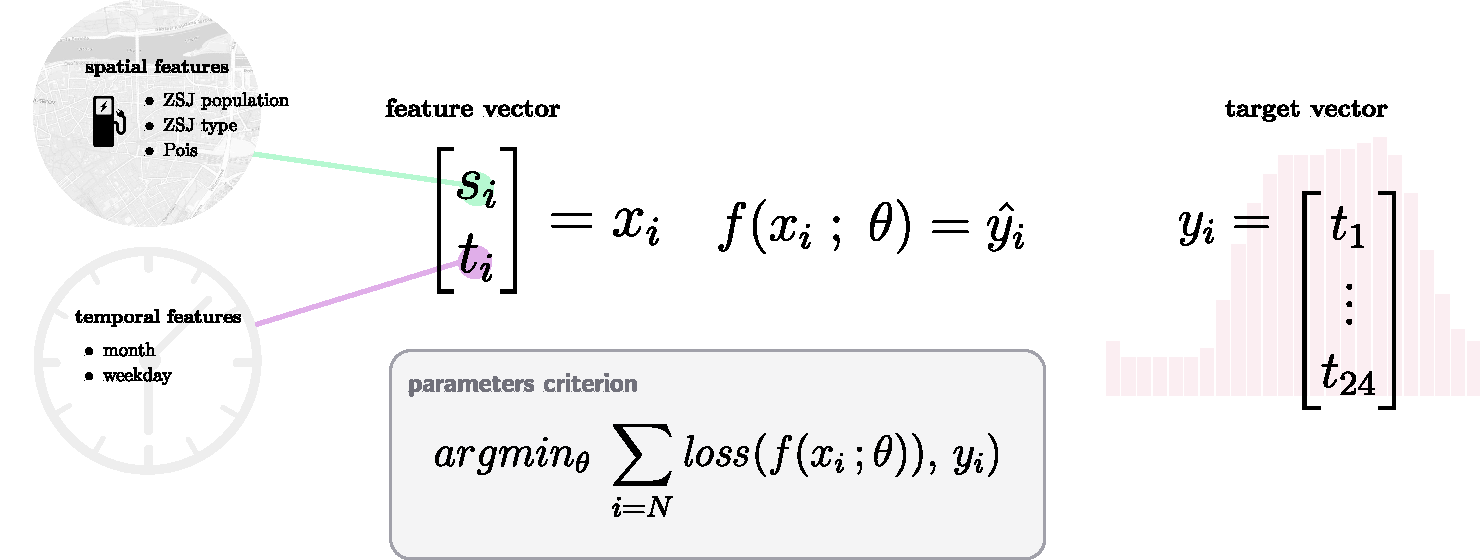
\includegraphics[width=1\textwidth]{diagram-detail}
    \caption[Problem modelling overview]{Problem approach overview}
\end{figure}
\todo[inline]{This figure should include a more detailed caption explaining the key components and their relationships. Consider adding labels to the diagram to make it more self-explanatory.}

In this chapter, we formulate the research problem of estimating electric vehicle charging demand and present our approach to solving it. We begin with a clear problem statement, followed by a detailed description of our feature engineering process. We then introduce our neural network architecture with latent profiles, which is designed to capture both temporal and spatial patterns in charging behavior. Finally, we explain our dataset splitting strategy, training procedure, and the baseline models used for comparative evaluation.

\todo[inline]{This introduction provides a good overview of the chapter structure, but should also briefly mention the rationale behind choosing a neural network with latent profiles over other potential approaches. Additionally, consider adding a paragraph that connects this chapter to the previous chapters, particularly how the data described in Chapter 4 informs the modeling approach.}

\section{Problem statement}

% \begin{marginfigure}
%     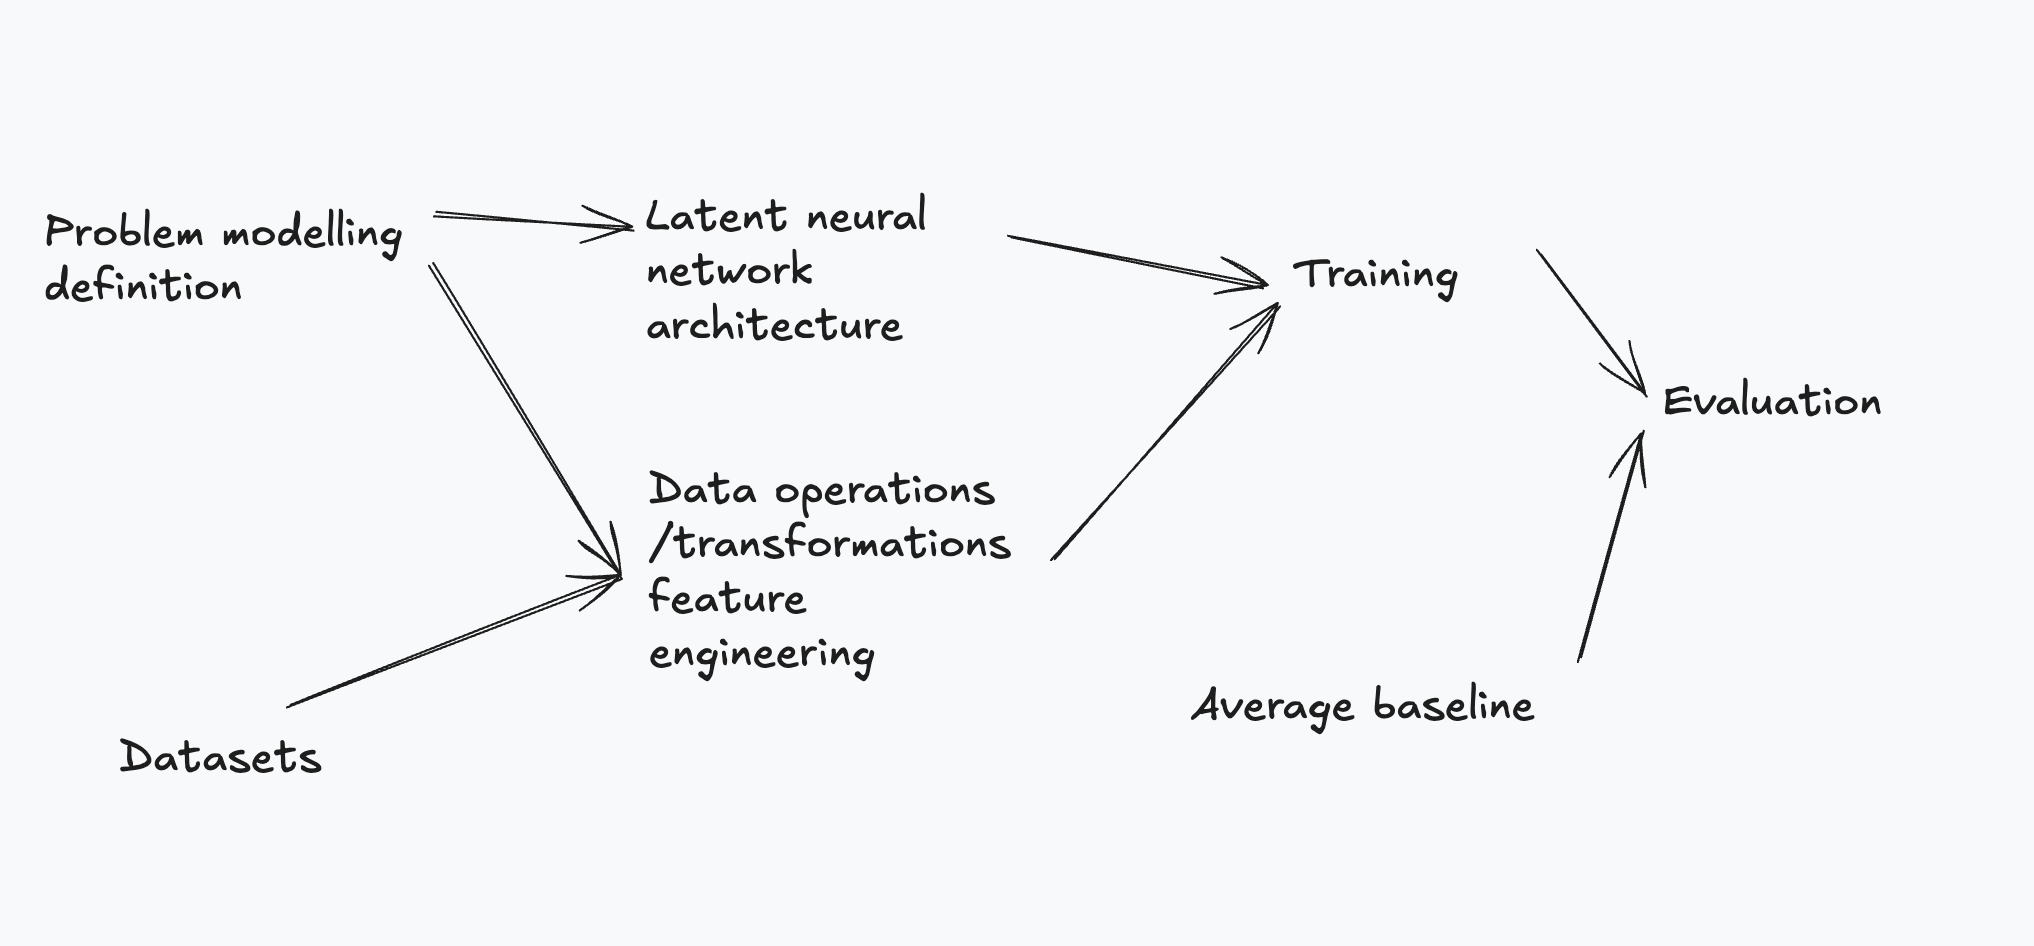
\includegraphics{diagram}
%     \caption[Problem modelling overview]{Chapter content overview.}
% \end{marginfigure}

Our primary objective is to estimate the \acrfull{APC} of electric vehicle charging stations based on a set of spatial and temporal features. Through this research, we aim to determine whether our data-driven approach is viable for predicting charging demand at new locations.

\todo[inline]{This problem statement should be expanded to include specific research questions that the study aims to answer. For example: "How accurately can spatial and temporal features predict charging demand patterns?" or "Which features are most influential in determining charging demand?"}

Formally, we define our model $f_\theta$ as a function that maps from a feature space to a target space:

\[
    f_{\theta}: X \rightarrow Y
\]

Where $X \subset \mathbb{R}^M$ represents the set of all feature vectors (with $M$ dimensions), and $Y \subset \mathbb{R}^{24}$ represents the set of all target vectors (hourly power consumption over a 24-hour period). The available data are split into \textit{training}, \textit{test}, and \textit{validation} sets, with the training set used to minimize the empirical risk. The details of this splitting strategy are explained in Section \ref{sec:dataset-split}.

\todo[inline]{Consider adding a brief discussion of the challenges and limitations of this problem formulation, such as the potential for overfitting, the difficulty of capturing complex temporal patterns, or the challenge of generalizing to new locations with different characteristics.}

The model function $f$ has trainable parameters $\theta$, which we optimize to minimize the following empirical risk:

\begin{equation}
    \mathit{loss_{total}}(f,\theta) = \frac{1}{P} \sum_{(x,y)\in\mathcal{T}} \alpha \cdot a_x + \beta \cdot b_x
\end{equation}

Where $P$ is the number of samples in the training set $\mathcal{T}$, and $\alpha$ and $\beta$ are weighting coefficients for the two components of our loss function:

\begin{equation}
    \begin{split}
        a_x & = \mathit{loss_{power}}
        (\left \lVert f(x_i;\theta) \right \rVert_{1}, \left \lVert y_i \right \rVert_{1}) \\
        b_x & = \mathit{loss_{norm}}
        (\frac{f(x_i;\theta)}{\left \lVert f(x_i;\theta) \right \rVert_{1}}, \frac{y_i}{\left \lVert y_i \right \rVert_{1}})
    \end{split}
\end{equation}

\todo[inline]{There appears to be a typo in the text: "inp predicting" should be "in predicting". Also, specify what specific loss functions (e.g., MSE, MAE) are used for loss power and loss norm.}

The first component, $a_x$, measures the error inp predicting the \acrfull{TDPC} using the $L1$ norm of the predicted and actual consumption vectors. The second component, $b_x$, measures the error in predicting the \acrfull{NDPC} by comparing the normalized predicted and actual consumption patterns. This dual-objective loss function aligns with our neural network architecture, which separately models the total power consumption and the normalized consumption pattern.

\todo[inline]{Explain the rationale for choosing this dual-objective loss function and how the values of alpha and beta were determined. Were they set empirically, through cross-validation, or based on domain knowledge? Also discuss how this loss function addresses the specific challenges of the charging demand prediction problem.}

The practical use case of our model is to help EV charging infrastructure planners answer the question: what will be the power consumption profile if a new \acrfull{CS} is placed at a specific location in Prague? Planners are particularly interested in understanding how consumption patterns vary with temporal factors\sidenote{e.g., how would a new charger at location $x$ perform on Thursdays of February}.

\section{Model features and feature engineering}

Our feature vector consists of both \textbf{temporal} and \textbf{spatial} components. Ideally, features regarding the charger's capabilities (particularly maximum power output) would also be included, as these would significantly influence average consumption. However, due to limitations in our current dataset, these features are not available. This limitation motivates our interest in estimating the \acrfull{NDPC}, which may be less dependent on the charger's maximum power output.

\todo[inline]{This is an important limitation that should be discussed more thoroughly. Consider adding a paragraph about how this limitation might affect model performance and what strategies could be employed in future work to address it. Also, provide evidence or reasoning for why NDPC might be less dependent on charger capabilities.}

The features in our model fall into two categories based on data type: categorical and numerical. We process these feature types as follows:

\textbf{Categorical features} are transformed using one-hot encoding. This technique converts a categorical feature with $n$ possible values into $n$ binary features, where each binary feature corresponds to one possible value. For each observation, exactly one of these binary features has the value 1, indicating the presence of that categorical value, while all others are 0.

\marginnote{For example, if we have a categorical feature "day of week" with 7 possible values (Monday through Sunday), one-hot encoding transforms this into 7 binary features: "is\_Monday", "is\_Tuesday", etc. If an observation occurs on Wednesday, then the "is\_Wednesday" feature would be 1, while all other day features would be 0. This transformation allows the model to properly handle categorical variables without imposing an arbitrary ordinal relationship between category values.}

In our model, categorical features such as day of the week, month, and location characteristics are one-hot encoded before being fed into the neural network. This ensures that the model can effectively learn from these categorical variables without imposing arbitrary numerical relationships.

\textbf{Numerical features} are standardized by subtracting the mean and dividing by the standard deviation. This normalization ensures all features are on a comparable scale, preventing features with larger magnitudes from dominating the learning process and helping achieve faster convergence during training.

The feature vector $x_i$ for each sample is constructed as follows:

\begin{equation}
    \renewcommand*{\arraystretch}{1.5}
    x_i = \begin{bmatrix}
        s_i^T \\
        t_i^T
    \end{bmatrix}
\end{equation}

Where $s_i$ represents the spatial features and $t_i$ represents the temporal features.

The \textbf{spatial features} vector $s_i$ is defined as:

\begin{equation}
    s_i = \begin{bmatrix}
        s_i^1  \\
        \vdots \\
        s_i^R
    \end{bmatrix}
\end{equation}

Table \ref{tab:spatial-features-table} provides a detailed overview of the spatial features used in our model.

\begin{table*}[h!]
    \def\arraystretch{1.5}
    \caption{Overview of spatial features used in the feature vector. The additional processing is described in Section \ref{sec:spatial-transformations}}
    \label{tab:spatial-features-table}
    \begin{tabular}{p{1cm} p{3.5cm} p{1.8cm} p{3.5cm} p{4.5cm}}
        \toprule
        \textbf{Index} & \textbf{Name}                                                       & \textbf{Type} & \textbf{Value from}                  & \textbf{Additional processing}                                                                                             \\
        \midrule
        $s_{1}$        & ZSJ population                                                      & numeric       & charger in ZSJ polygon               & normalization by the polygon area                                                                                          \\
        $s_{2:10}$     & ZSJ type                                                            & categorical   & charger in ZSJ polygon               & one-hot encoding                                                                                                           \\
        $s_{11}$       & ZSJ number of addresses                                             & numeric       & charger in ZSJ polygon               & normalization by the polygon area                                                                                          \\
        $s_{12}$       & Number of people commuting into the district from inside Prague     & numeric       & charger in the district polygon      & normalization by the polygon area                                                                                          \\
        $s_{13}$       & Number of people commuting into the district from outside of Prague & numeric       & charger in the district polygon      & normalization by the polygon area                                                                                          \\
        $s_{14:162}$   & Points of Interest                                                  & numeric       & number of PoIs by euclidean distance & importance calculation (value of single PoI is 1 if its distance from charger is 0, 0 if it is of distance 2km or further) \\
        \bottomrule
    \end{tabular}
\end{table*}

The \textbf{temporal features} vector $t_i$ is defined as:

\begin{equation}
    t_i = \begin{bmatrix}
        t_i^1  \\
        \vdots \\
        t_i^P
    \end{bmatrix}
\end{equation}

Table \ref{tab:temporal-features-table} provides a detailed overview of the temporal features used in our model.

\begin{table*}[h!]
    \caption{Overview of temporal features used in the feature vector.}
    \label{tab:temporal-features-table}
    \begin{tabular}{p{1cm} p{3.5cm} p{1.8cm} p{3.5cm} p{4.5cm}}
        \toprule
        \textbf{Index} & \textbf{Name}   & \textbf{Type} & \textbf{Value from} & \textbf{Additional processing} \\
        \midrule
        $t_{1:7}$      & day of the week & categorical   & \acrfull{APC}       & one-hot encoding               \\
        $t_{8:19}$     & month           & categorical   & \acrfull{APC}       & one-hot encoding               \\
        \bottomrule
    \end{tabular}
\end{table*}

\section{Architecture of the Latent Neural Network}

Our machine learning problem formulation allows for various potential solutions, particularly within the class of neural networks. Before introducing our specific architecture, let's briefly review the fundamentals of neural networks.

\todo[inline]{While the neural network overview is well-written, it may be unnecessary for a master's thesis, as readers are likely familiar with basic neural network concepts. Consider condensing this paragraph and focusing more on the specific innovations in your architecture.}

Neural networks are computational models consisting of layers of interconnected nodes or "neurons" that process information. A typical neural network contains an input layer that receives data, one or more hidden layers that perform computations, and an output layer that produces the final result. Each connection between neurons has an associated weight that is adjusted during the training process. Information flows through the network via activation functions, which introduce non-linearity and allow the network to learn complex patterns. The training process involves feeding the network with labeled examples and using optimization algorithms, typically variants of gradient descent, to minimize a loss function by adjusting the weights. Backpropagation is the primary algorithm used to calculate gradients and update weights efficiently.

For our specific problem, we propose a neural network with latent profiles, as illustrated in Figure \ref{fig:nn-latent}. The key innovation in our architecture is the construction of a latent profile matrix $R \in \mathbb{R}^{24 \times K}$, where $K$ is the number of latent profiles. The network learns these profiles and predicts how they should be combined to generate the final consumption pattern for a given location and time period.

\todo[inline]{Provide more context for the latent profiles approach. What inspired this architecture? Are there similar approaches in the literature? How does this approach specifically address the challenges of charging demand prediction? Also, explain how the value of K was determined.}

\newpage

The network utilizes the following layers:

\newcommand{\nnmodule}[3]{%
    \begin{marginfigure}[1cm]
        \centering
        \includegraphics[width=1.8cm]{#2}
    \end{marginfigure}
    \item \textbf{#1} \\
    #3
    \vspace{2mm}
}


\begin{itemize}
    \item[] \textbf{Trainable layers:}
          \begin{itemize}
              \nnmodule{Fully connected (Linear transformation)}{nn-modules/fully-conn.pdf}{%
                  $\text{Linear}^n_m(x) = W x + b$ \\
                  $\text{Linear}^n_m: \mathbb{R}^n \rightarrow \mathbb{R}^m \; , \;
                      W \in \mathbb{R}^{m \times n} \; , \;
                      b \in \mathbb{R}^m$ \\
                  $W, b$ are learnable parameters \\

                  \vspace{2mm}

                  This is a standard linear transformation that maps input vectors to output vectors through a weight matrix and bias vector.
              }

              \nnmodule{Latent vectors (Embedding)}{nn-modules/grad-parameter.pdf}{%
                  $\text{LatentVec}_K = R$ \\
                  $\text{LatentVec}_K: \emptyset \rightarrow \mathbb{R}^{24 \times K}$ \\
                  $R$ is learnable

                  \vspace{2mm}

                  This layer represents our latent profiles matrix, which contains $K$ different 24-hour consumption patterns that the network learns during training.
              }

          \end{itemize}

    \item[] \textbf{Non-parametric operations:}
          \begin{itemize}
              \nnmodule{Softplus (Smooth activation)}{nn-modules/softplus.pdf}{%
                  $f(x) = \ln(1 + e^x)$ \\
                  $f: \mathbb{R} \rightarrow \mathbb{R}^+$

                  \vspace{2mm}

                  Softplus is a smooth approximation of the ReLU activation function. It ensures that the output is always positive, which is appropriate for our case since power consumption cannot be negative.
              }

              \nnmodule{Normalization}{nn-modules/norm.pdf}{%
                  $\text{Norm}(x) = \frac{x}{\|x\|_2}$ \\
                  $\text{Norm}: \mathbb{R}^n \rightarrow \{y \in \mathbb{R}^n : \|y\|_2 = 1\}$ \\
                  input dimension matches output dimension \\

                  \vspace{2mm}

                  This operation normalizes vectors to have unit L2 norm. We use it to normalize our latent profiles and to compute the normalized daily power consumption pattern.
              }

              \nnmodule{Leaky-relu}{nn-modules/leaky-relu.pdf}{%
                  $\text{LReLU}(x) = \begin{cases}
                          x        & \text{if } x > 0    \\
                          \alpha x & \text{if } x \leq 0
                      \end{cases}$ \\
                  $\text{LReLU}: \mathbb{R} \rightarrow \mathbb{R} \; , \; \alpha \text{ is a hyperparameter}$ \\

                  \vspace{2mm}

                  Leaky ReLU is an extension of the standard ReLU activation function that allows a small gradient when the unit is not active. In this work, there is no clear motivation for its use over tanh or standard ReLU.
              }
          \end{itemize}
\end{itemize}

\vspace{5mm}

\newpage

These layers are combined to form three functional modules, each with a specific purpose in our neural network architecture:

\begin{itemize}
    \item[] \textbf{Network modules:}
          \begin{itemize}
              \nnmodule{f module (Latent profile probabilities)}{nn-modules/f-module.pdf}{%
                  $f: \mathbb{R}^d \rightarrow \mathbb{R}^K$ \\
                  $f = \text{Softmax} \circ \text{Linear}_{K} \circ \text{LeakyReLU} \circ \text{Linear}_{64} \circ \text{LeakyReLU} \circ \text{Linear}_{h}$ \\
                  Where $d$ is feature size, $h$ is hidden size, and $K$ is latent profiles count \\
                  Outputs normalized weights for latent profiles

                  \vspace{3mm}

                  The purpose of this module is to predict the contribution of individual latent profiles to the resulting normalized consumption pattern. In other words, this module estimates the daily rhythm of the charger without considering the actual total power. The input is a feature vector, which is transformed by two linear layers with LeakyReLU activations. The output is a vector of $K$ values transformed by softmax to ensure the sum equals 1, representing the mixing weights for the latent profiles.
              }

              \nnmodule{g module (Total power)}{nn-modules/g-module.pdf}{%
                  $g: \mathbb{R}^d \rightarrow \mathbb{R}$ \\
                  $g = \text{Linear}_{1} \circ \text{LeakyReLU} \circ \text{Linear}_{32} \circ \text{LeakyReLU} \circ \text{Linear}_{h_g}$ \\
                  Where $d$ is feature size and $h_g$ is hidden size for g module

                  \vspace{3mm}

                  This module predicts the total power consumption for the given temporal pattern and location. It consists of three linear layers joined with LeakyReLU activations. Its input is a feature vector, and it outputs a single scalar. This scalar is multiplied with the combined output of the h module to obtain the final prediction, effectively scaling the normalized consumption pattern to the appropriate magnitude.
              }

              \nnmodule{h module (Latent profiles)}{nn-modules/h-module.pdf}{%
                  $h(\mathbf{x}) = f(\mathbf{x}) \cdot R^T$ \\
                  $h: \mathbb{R}^d \rightarrow \mathbb{R}^{24}$ \\
                  Where $R \in \mathbb{R}^{24 \times K}$ is the normalized latent profiles matrix \\
                  $24$ is the time granularity (hours in a day), $K$ is latent profiles count

                  \vspace{3mm}

                  The h module combines the outputs of the f module with the latent profiles matrix R to produce a normalized 24-hour consumption pattern. It takes the weights predicted by the f module and computes a weighted sum of the latent profiles. This module effectively translates the abstract latent space representation into a concrete hourly consumption pattern, capturing the temporal dynamics of charging behavior at the given location.
              }
          \end{itemize}
\end{itemize}

\vspace{5mm}

\newpage

The outputs of the h and f modules are combined as follows:

\begin{equation}
    \begin{split}
         & \text{Combine}(R,p) = \sum_{i=1}^K p_i \, R_i                                            \\
         & \text{Combine}: \mathbb{R}^{24 \times K} \times \mathbb{R}^K \rightarrow \mathbb{R}^{24}
    \end{split}
\end{equation}

This combined output is then multiplied by the scalar from the g module to produce the final prediction of hourly power consumption.

\begin{figure}[hb]
    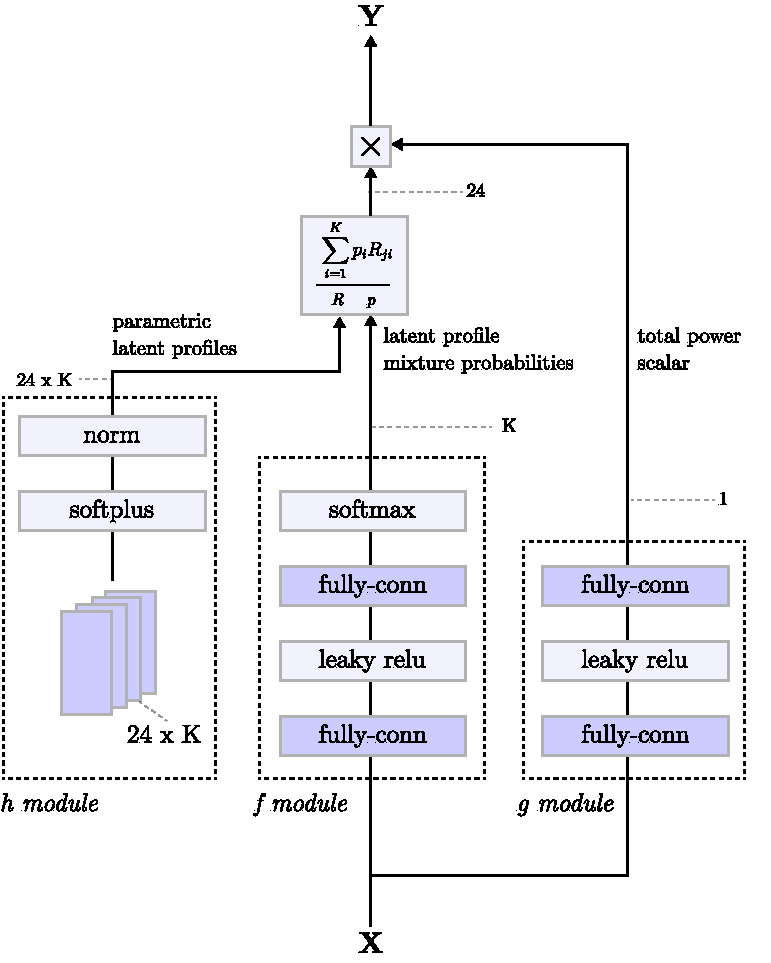
\includegraphics[width=0.8\textwidth]{nn-latent-architecture.pdf}
    \caption[Latent Neural Network Architecture]{Latent neural network architecture. Light blue rectangles denote NN layers without trainable parameters, while blue denotes layers with parameters learned by SGD. Notation borrowed from Fleuret's book "Little Book of Deep Learning"}
    \label{fig:nn-latent}
\end{figure}

The model is implemented in Python using the PyTorch library
\sidecite{paszke2019pytorchimperativestylehighperformance}.

\newpage


\section{Dataset splitting}
\label{sec:dataset-split}

Our dataset splitting strategy is designed to evaluate the model's ability to generalize to new locations, which is crucial for our use case of predicting demand for new charging stations.

We split our data into three sets: training, test, and validation. However, we cannot simply randomly assign samples to these sets because of the hierarchical nature of our data. Specifically, one physical location may have multiple charging points (CPs) within a charging station (CS), and each CP may have multiple average power consumption (APC) measurements for various temporal patterns (TP). There might be high correlation between measurements from the same location, which would lead to data leakage if we split randomly.

To address this issue, we split the data based on location. Features for each unique location can only be present in one of the sets. This ensures that when we evaluate our model on the test or validation set, it is truly being tested on locations it has never seen during training.

% \begin{equation}
%     \begin{split}
%         \textit{train}:      \; \mathcal{T} & = ((x_i, y_i) \in X \times Y |\, i = 1,\dots, P) \\
%         \textit{test}:       \; \mathcal{S} & = ((x_i, y_i) \in X \times Y |\, i = 1,\dots, R) \\
%         \textit{validation}: \; \mathcal{V} & = ((x_i, y_i) \in X \times Y |\, i = 1,\dots, O)
%     \end{split}
% \end{equation}

The three datasets serve distinct purposes in our research:

\begin{itemize}
    \item \textbf{Train dataset} is used for training the model using \acrlong{SGD} for empirical risk minimization.
          \begin{equation}
              \label{eq:train}
              \textit{train}: \; \mathcal{T} = \{(x_i, y_i) \in X \times Y |\, i = 1,\dots, P\}
          \end{equation}
          \vspace{3mm}


    \item \textbf{Test dataset} is used for inspecting the model's performance on unseen data and tuning hyperparameters. It provides an estimate of the true model risk.

          \begin{equation}
              \label{eq:test}
              \textit{test}: \; \mathcal{S} = \{(x_i, y_i) \in X \times Y |\, i = 1,\dots, R\}
          \end{equation}
          \vspace{3mm}
    \item \textbf{Validation dataset} is used to obtain the final model risk assessment on a model with already trained parameters and chosen hyperparameters.
          \begin{equation}
              \label{eq:validation}
              \textit{validation}: \; \mathcal{V} = \{(x_i, y_i) \in X \times Y |\, i = 1,\dots, O\}
          \end{equation}
\end{itemize}

\section{Training procedure}

To train our neural network model, we utilize the standard PyTorch training procedure with mini-batch \acrfull{SGD} optimization. The model is trained iteratively over multiple epochs, with early stopping implemented to prevent overfitting.

We selected a batch size of Y, and the model typically required approximately X epochs with early termination before it began to overfit the training dataset. These hyperparameters were determined through experimentation on the test set.

\todo[inline]{Replace the placeholder values X and Y with the actual batch size and typical number of epochs. Also, provide more details about the optimization process, including the specific optimizer used (e.g., Adam, SGD with momentum), learning rate, and any learning rate scheduling. Describe the early stopping criteria in detail.}

\subsection{Training dashboard}

To provide visibility into the training process, we developed a graphical user interface dashboard using the Python library Rerun \sidecite{Rerun}. This dashboard allows real-time inspection of the training process, including:

\begin{itemize}
    \item Plots of training and validation loss over time
    \item Visualization of the learned latent profiles
    \item Prediction results for random samples from the validation dataset
\end{itemize}

\begin{figure}[hb]
    \begin{tabular}{cc}
        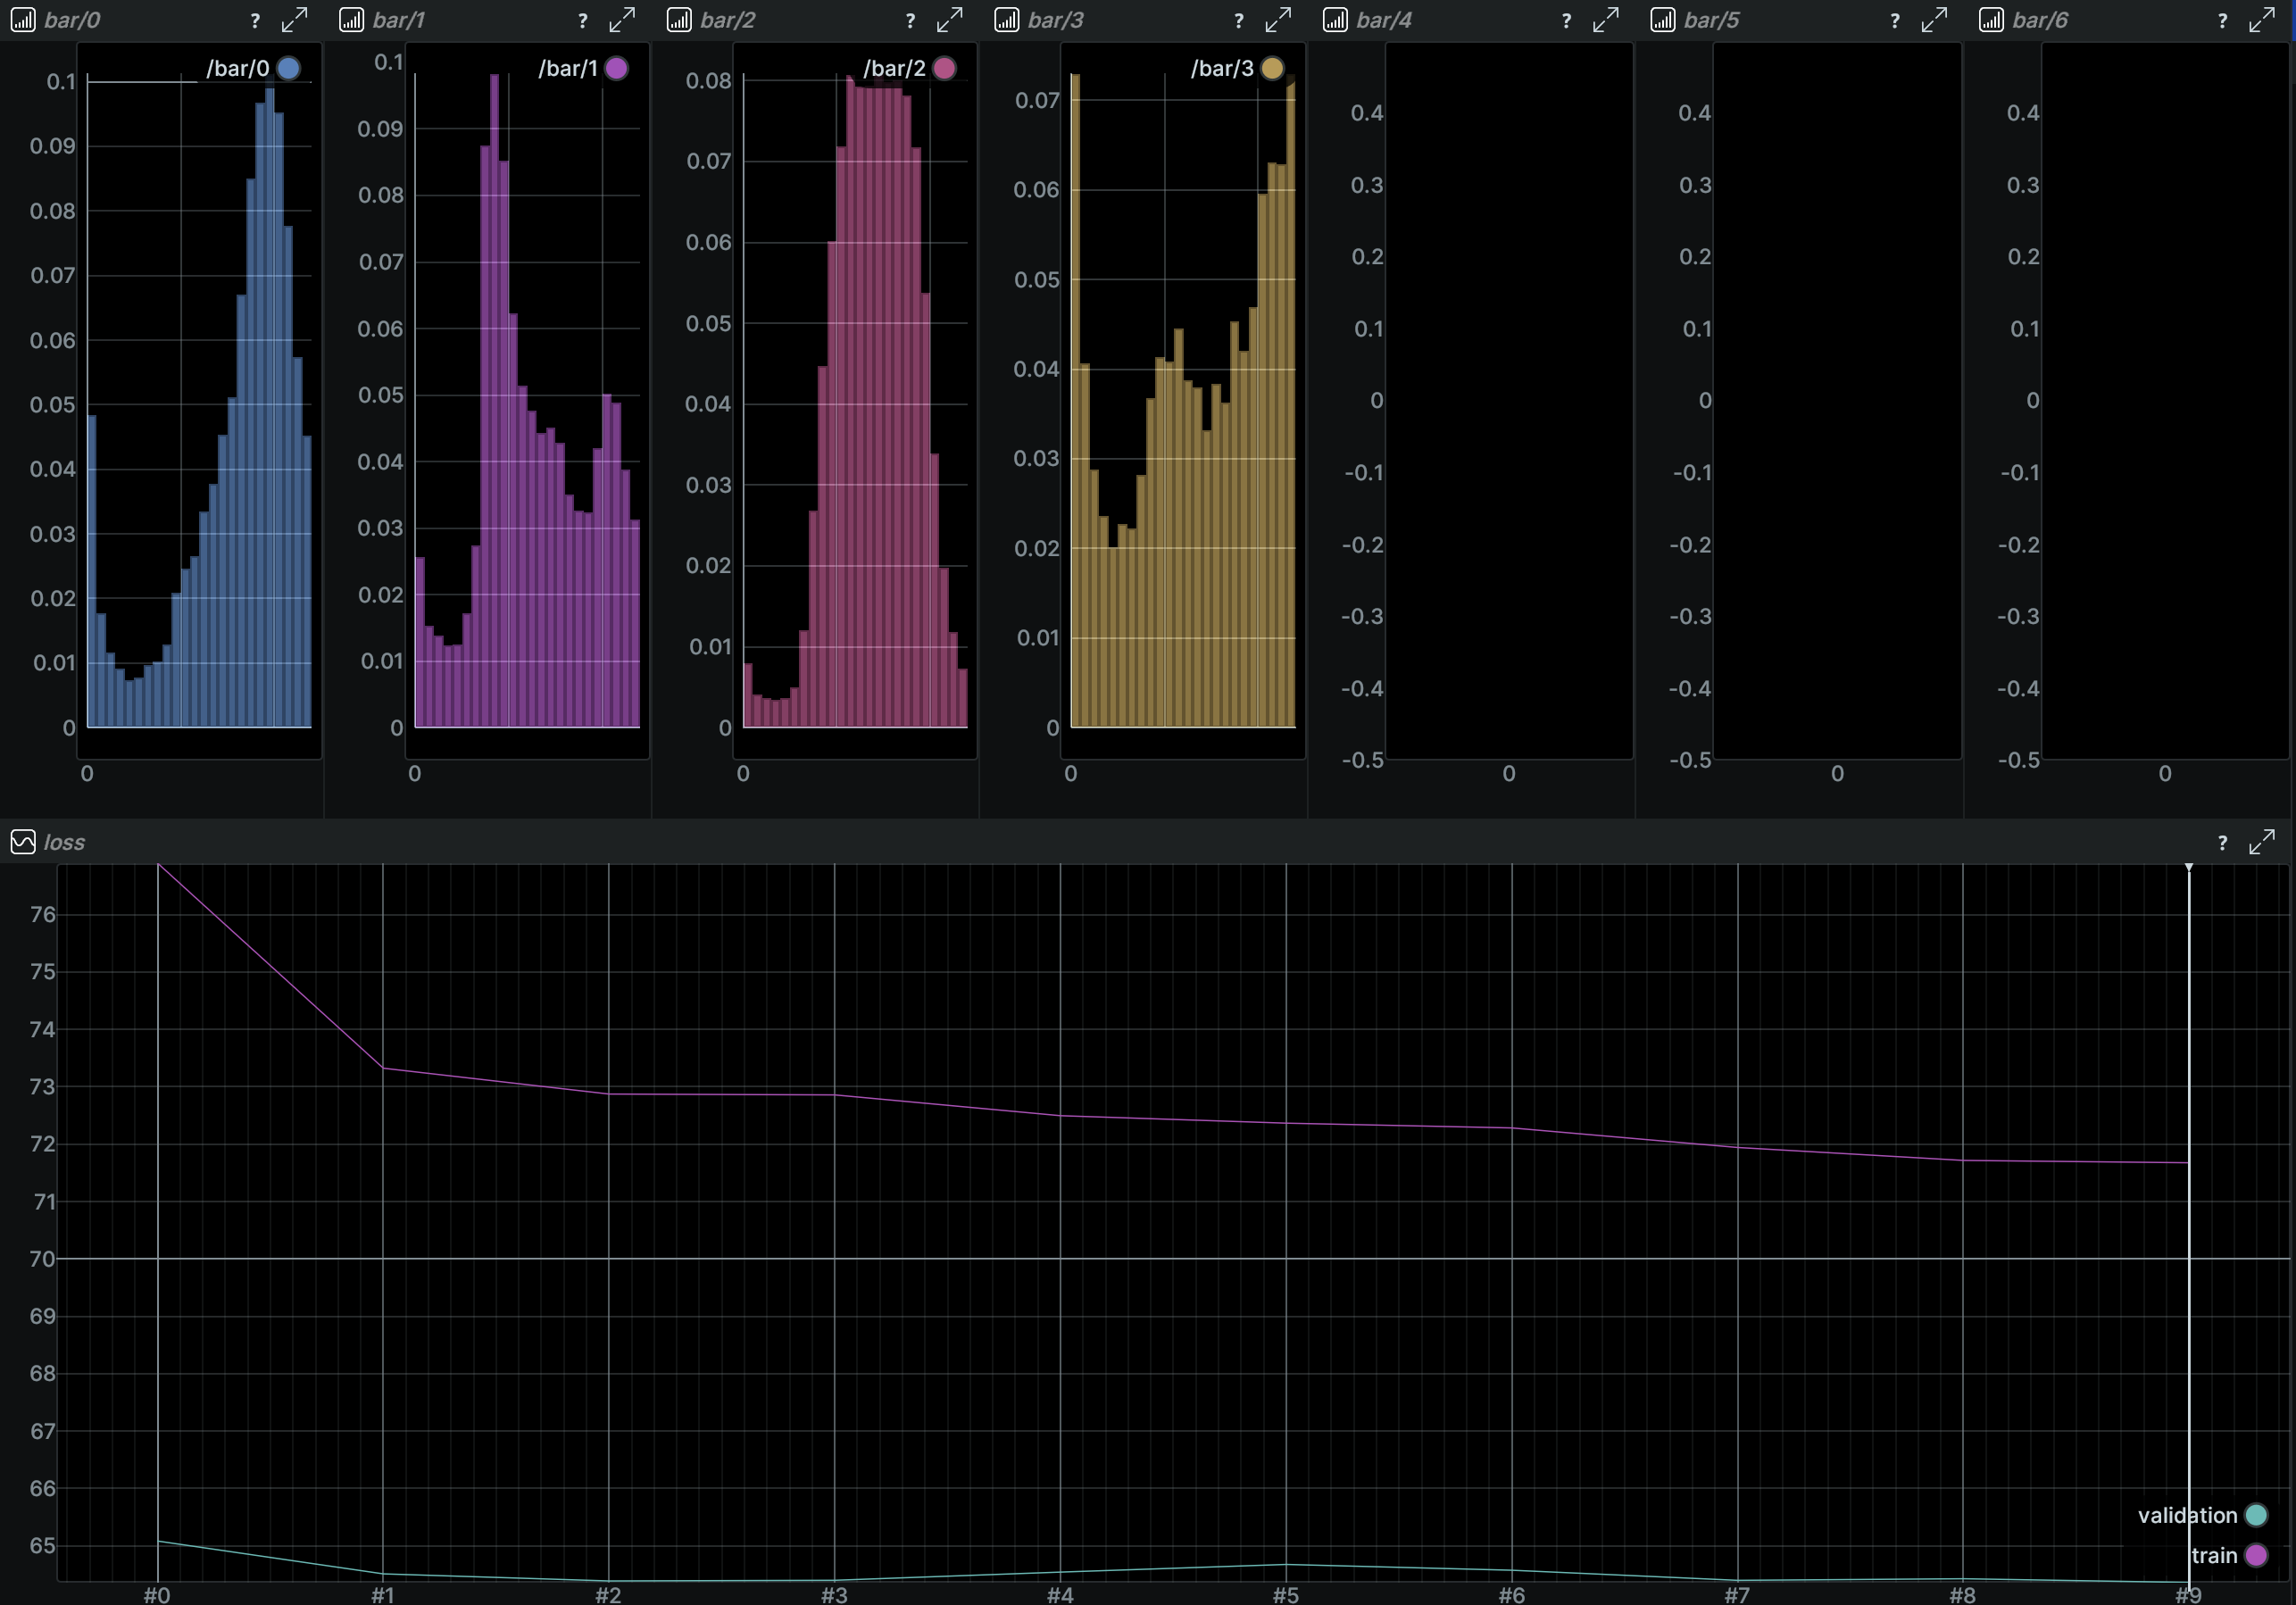
\includegraphics[width=0.7\textwidth]{rerun-train-validation.png} &
        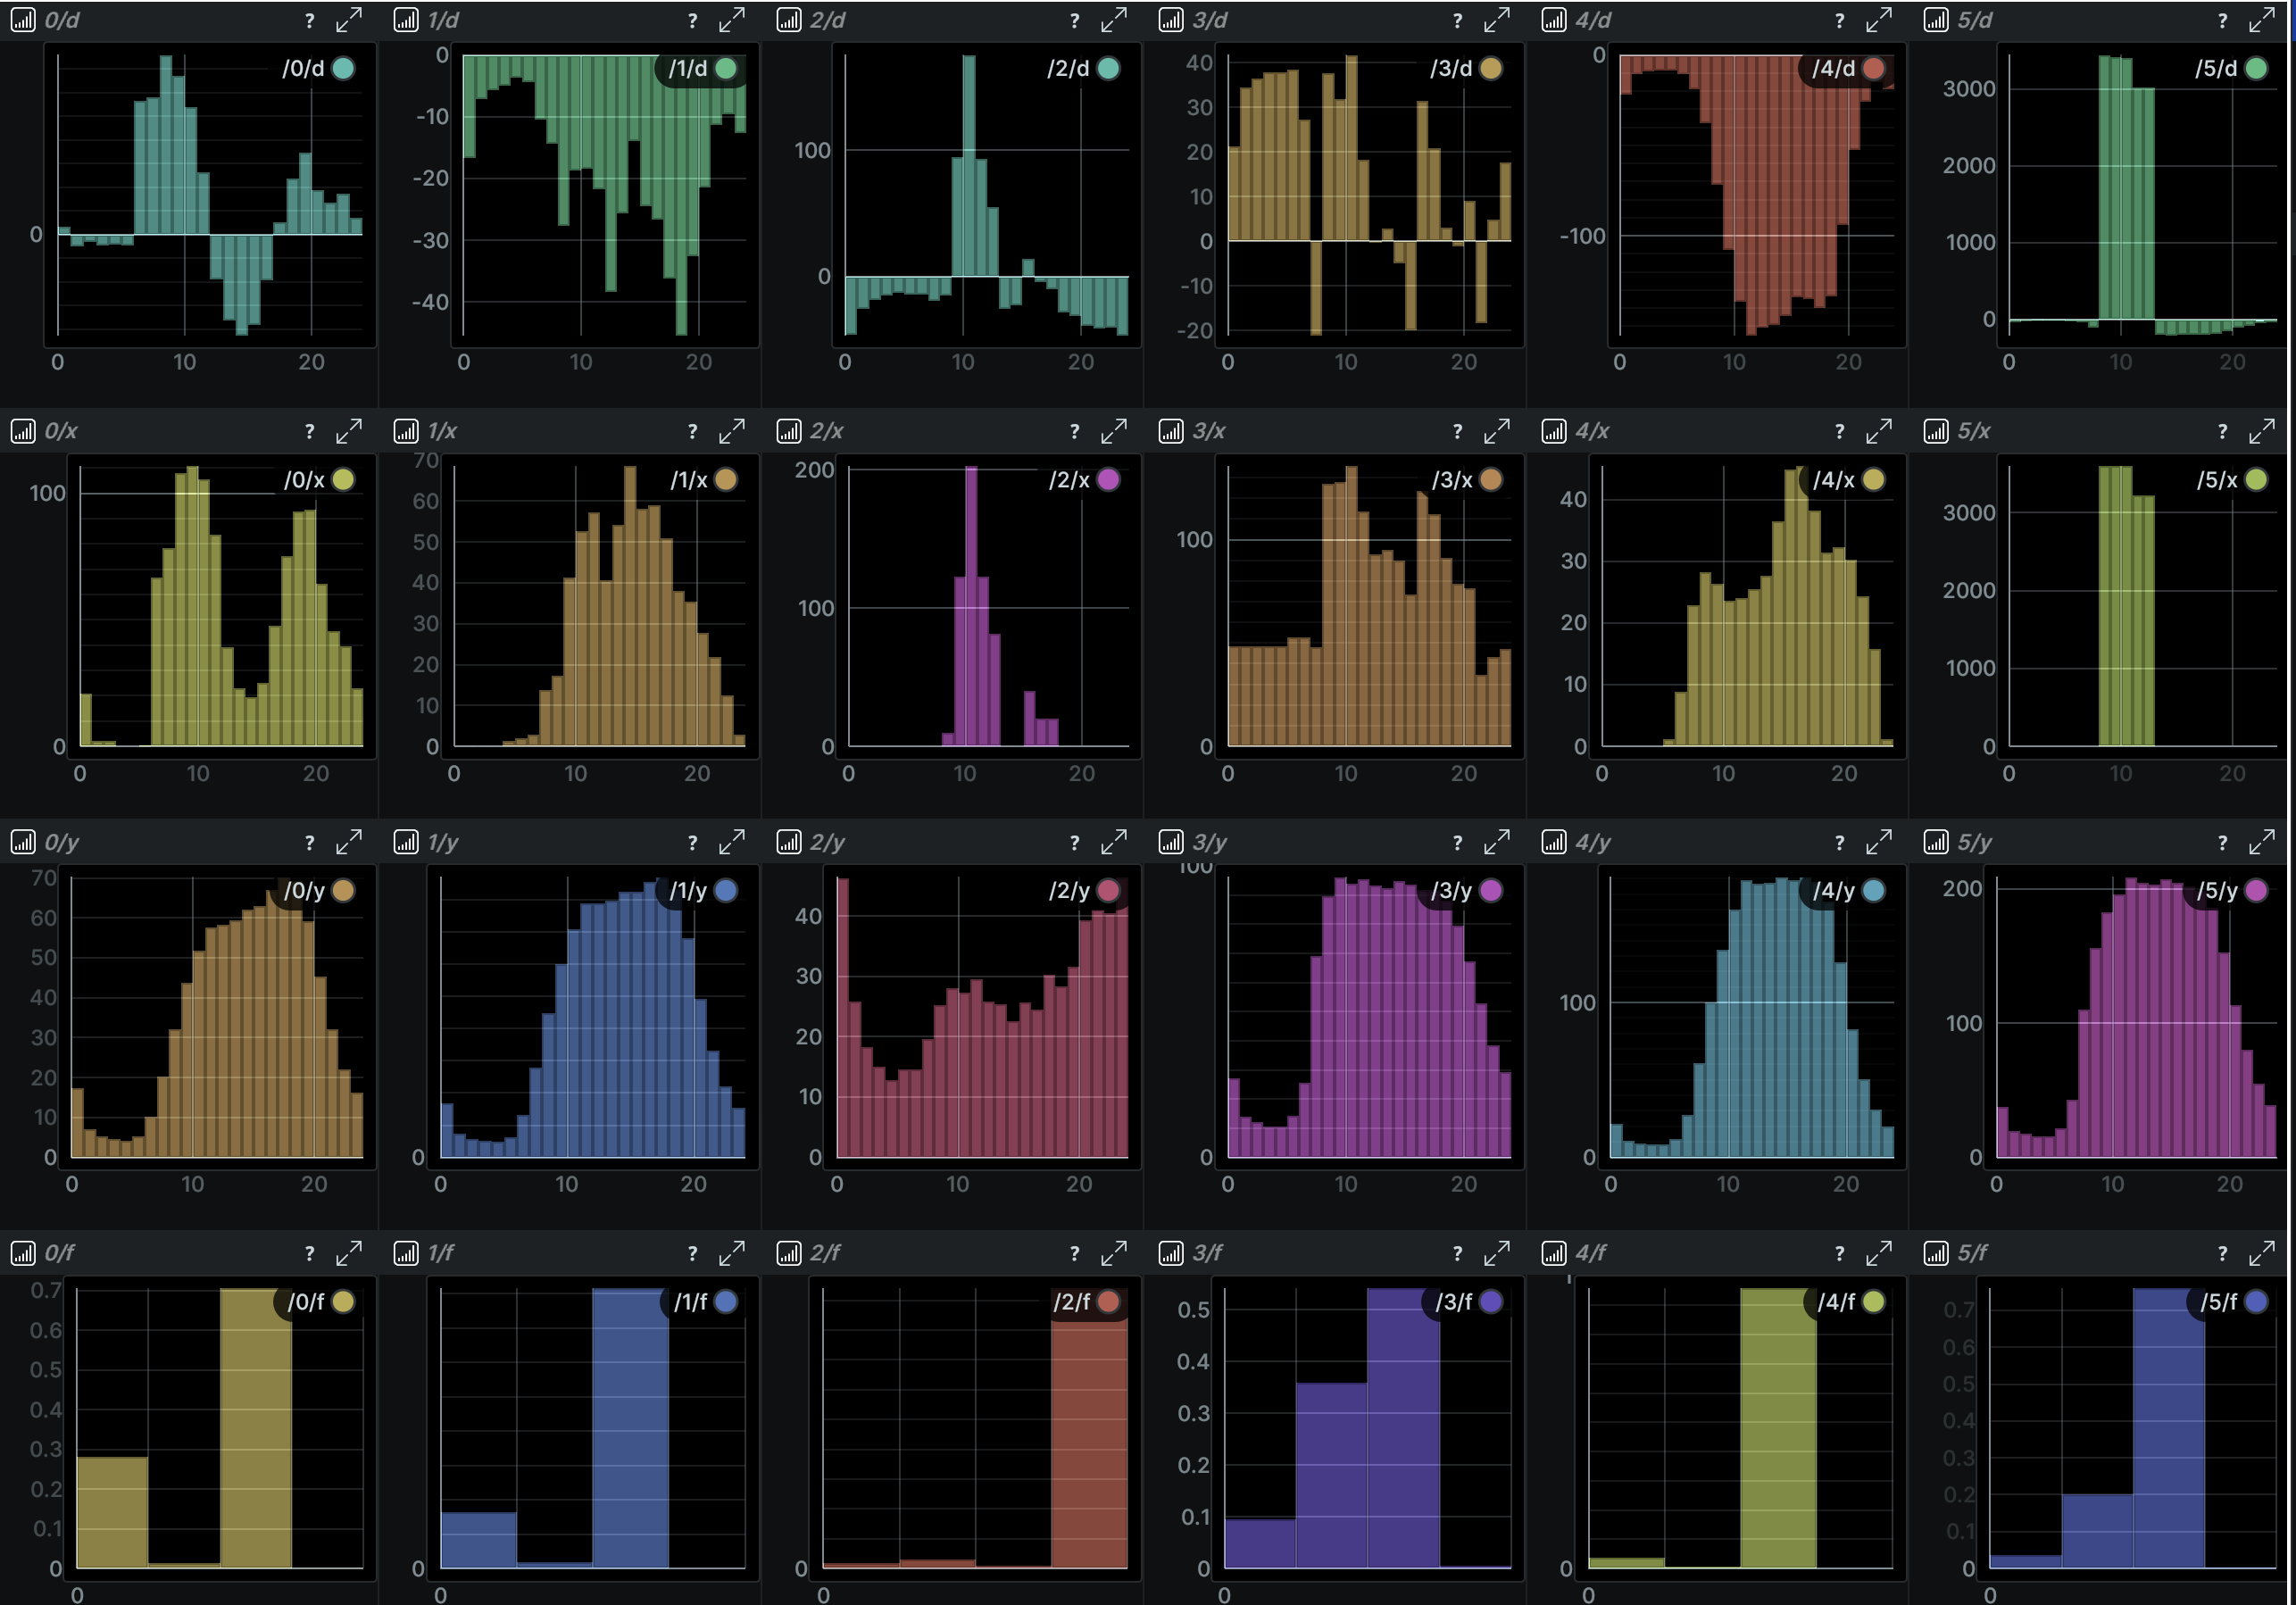
\includegraphics[width=0.7\textwidth]{rerun-predictions.png}
    \end{tabular}
    \caption{Rerun visualization dashboard showing training/validation loss (left) and model predictions (right).}
\end{figure}


\section{Other models for quantitative comparison}

To evaluate the effectiveness of our latent neural network approach, we compare it quantitatively with other machine learning models. The results from this comparison can either motivate further research with our model or indicate that simpler approaches may be sufficient.

One challenge in this comparison arises from our custom loss function, which combines two L1 losses. The baseline models are trained to minimize standard L1 loss, which might seem to create an unfair comparison. However, we provide more detailed analysis of this issue in Chapter \ref{ch:results}.

\todo[inline]{This section should explain why the specific baseline models (Average, Linear regression, XGBoost) were chosen. What makes them appropriate comparisons for your approach? Also, discuss how you addressed the challenge of comparing models with different loss functions to ensure a fair comparison.}

The models we use for comparison are:

\begin{itemize}
    \item \textbf{Average} - The simplest baseline, which takes the average over all feature vectors in the dataset and uses that value for all predictions. Both the train and test datasets $\mathcal{T}$ and $\mathcal{S}$ are utilized for this "model." It does not take into account the input features and uses a single value for all predictions.

          The implementation is straightforward:
          \begin{equation}
              \begin{split}
                   & f_{\mathcal{D}}(z) = \frac{1}{|\mathcal{D}|} \sum_{(x,\_) \in \mathcal{D}} x \\
                   & f: \mathbb{R}^m \rightarrow \mathbb{R}^n                                     \\
                   & n,m \in \mathbb{N}, \mathcal{D} \in (X \times Y)^p, p \in \mathbb{N}
              \end{split}
          \end{equation}


    \item \textbf{Linear regression} - A standard linear model that learns a linear mapping from input features to output predictions.

          We use the implementation from the Python library Scikit-Learn \sidecite{scikit-learn}:
          \begin{equation}
              \begin{split}
                   & f(z) = \alpha + \beta z                                    \\
                   & f: \mathbb{R}^m \rightarrow \mathbb{R}^n                   \\
                   & \alpha \in \mathbb{R}^n, \beta \in \mathbb{R}^{n \times m}
              \end{split}
          \end{equation}
    \item \textbf{XGBoost} - A scalable end-to-end tree boosting system \sidecite{Chen_2016}.
\end{itemize}

The performance of these models is compared with our latent neural network based on mean absolute error and mean square error for three metrics: \acrlong{APC} (hourly consumption), \acrlong{TDPC} (total daily consumption), and \acrlong{NDPC} (normalized daily consumption pattern).
